\section{Исследование управляемости}

Рассматриваем систему:
\begin{equation*}
    \dot x=Ax+Bu,\quad
    A=\begin{bmatrix}
        -1 & 1 & 0 \\ -2 & -4 & -1 \\ 2 & 2 & -1
    \end{bmatrix},\quad
    B=\begin{bmatrix}
        2 \\ 3 \\ -1
    \end{bmatrix},\quad
    x_1=\begin{bmatrix}
        1 \\ -3 \\ 3
    \end{bmatrix}.
\end{equation*}

\subsection{Исследование управляемости}

Найдем матрицу управляемости:
\begin{equation*}
    U=[B\quad AB\quad A^2B]=
    \begin{bmatrix}
        2 & 1 & -16 \\ 3 & -15 & 47 \\ -1 & 11 & -39
    \end{bmatrix}.
\end{equation*}
Матрица полноранговая, следовательно \textbf{система управляема}.

Спектр матрицы $A$:
$$\sigma(A)=\{ -2 + j; -2-j; -2\},$$
тогда матрицы Хаутуса ($[A-\lambda_iI\quad B]$) соответственно:
\begin{equation*}
    \begin{bmatrix}
        1-j&1&0&2\\-2&-2-j&-1&3\\2&2&1-j&-1
    \end{bmatrix},\quad 
    \begin{bmatrix}
        1+j&1&0&2\\-2&-2+j&-1&3\\2&2&1+j&-1
    \end{bmatrix},\quad
    \begin{bmatrix}
        1 & 1 & 0 & 2 \\
        -2 & -2 & -1 & 3 \\
        2 & 2 & 1 & -1
    \end{bmatrix}.
\end{equation*}
Все они трехранговые, \textbf{что удовлетворяет критерию Хаутуса управляемой системы}.

Жорданова форма матрицы $A$ и $P^{-1}B$:
\begin{equation*}
    A =\begin{bmatrix}
        
-2&	   0&	   0\\
0&	  -2&	   -1\\
0&	   1&	  -2\\

    \end{bmatrix},\quad
    P^{-1}B=\begin{bmatrix}
        2.0000 \\ -0.7071 \\ -6.3640
    \end{bmatrix}.
\end{equation*}
Как видно, система в Жордановой форме полностью управляема, а значит и \textbf{исходная система
полностью управляема}.

Итого, все три критерия сошлись на том, что система полностью управляема.

\subsection{Грамиан}

Найдем Грамиан управляемости системы относительно времени $t_1=3$:
\begin{equation*}
    P(3)=\int_{0}^{3}e^{At}BB^Te^{A^Tt}dt=
    \begin{bmatrix}
        2.2838  &  0.2838  &  1.1868 \\
        0.2838   & 1.1735  & -0.7618 \\
        1.1868  & -0.7618  &  1.3500
    \end{bmatrix}.
\end{equation*}
Его спектр:
\begin{equation*}
    \sigma(P(3))=\{ 0.0034;\ 
    3.1144;\ 
    1.6894\},
\end{equation*}
все числа положительны, а значит $det(P(3))=\lambda_1\cdot\lambda_2\cdot\lambda_3>0$ и
можно найти управление, которое переводит систему из $x(0)=0$ в $x(3) = x_1$.

\subsection{Управление}

Чтобы перевести систему из $x(0)=0$ в $x(3)=x_1$, достаточно взять программное управление:
\begin{multline*}
    u(t) = B^T e^{A^T(3 - t)} P(3)^{-1} x_1 = \\ =
    \begin{bmatrix}
        2 & 3 & -1
    \end{bmatrix}\cdot
    \exp\left( \begin{bmatrix}
        -1 & -2 & 2 \\ 
         1 & -4 & 2 \\ 
         0 & -1 & -1
    \end{bmatrix}\cdot(3 - t) \right)\cdot
    \begin{bmatrix}
        2.2838  &  0.2838  &  1.1868 \\
        0.2838   & 1.1735  & -0.7618 \\
        1.1868  & -0.7618  &  1.3500
    \end{bmatrix}^{-1}
    \begin{bmatrix}
        1 \\ -3 \\ 3
    \end{bmatrix}=\\
    =-e^{2t-6}\left(31.4860\sin\left(t-3\right)-6.3896\cos\left(t-3\right)+13.4230\right)
\end{multline*}

Смоделируем систему и данное управление, результаты приведены на рисунке \ref{fig:task1}.
\begin{figure}[H]
    \centering
    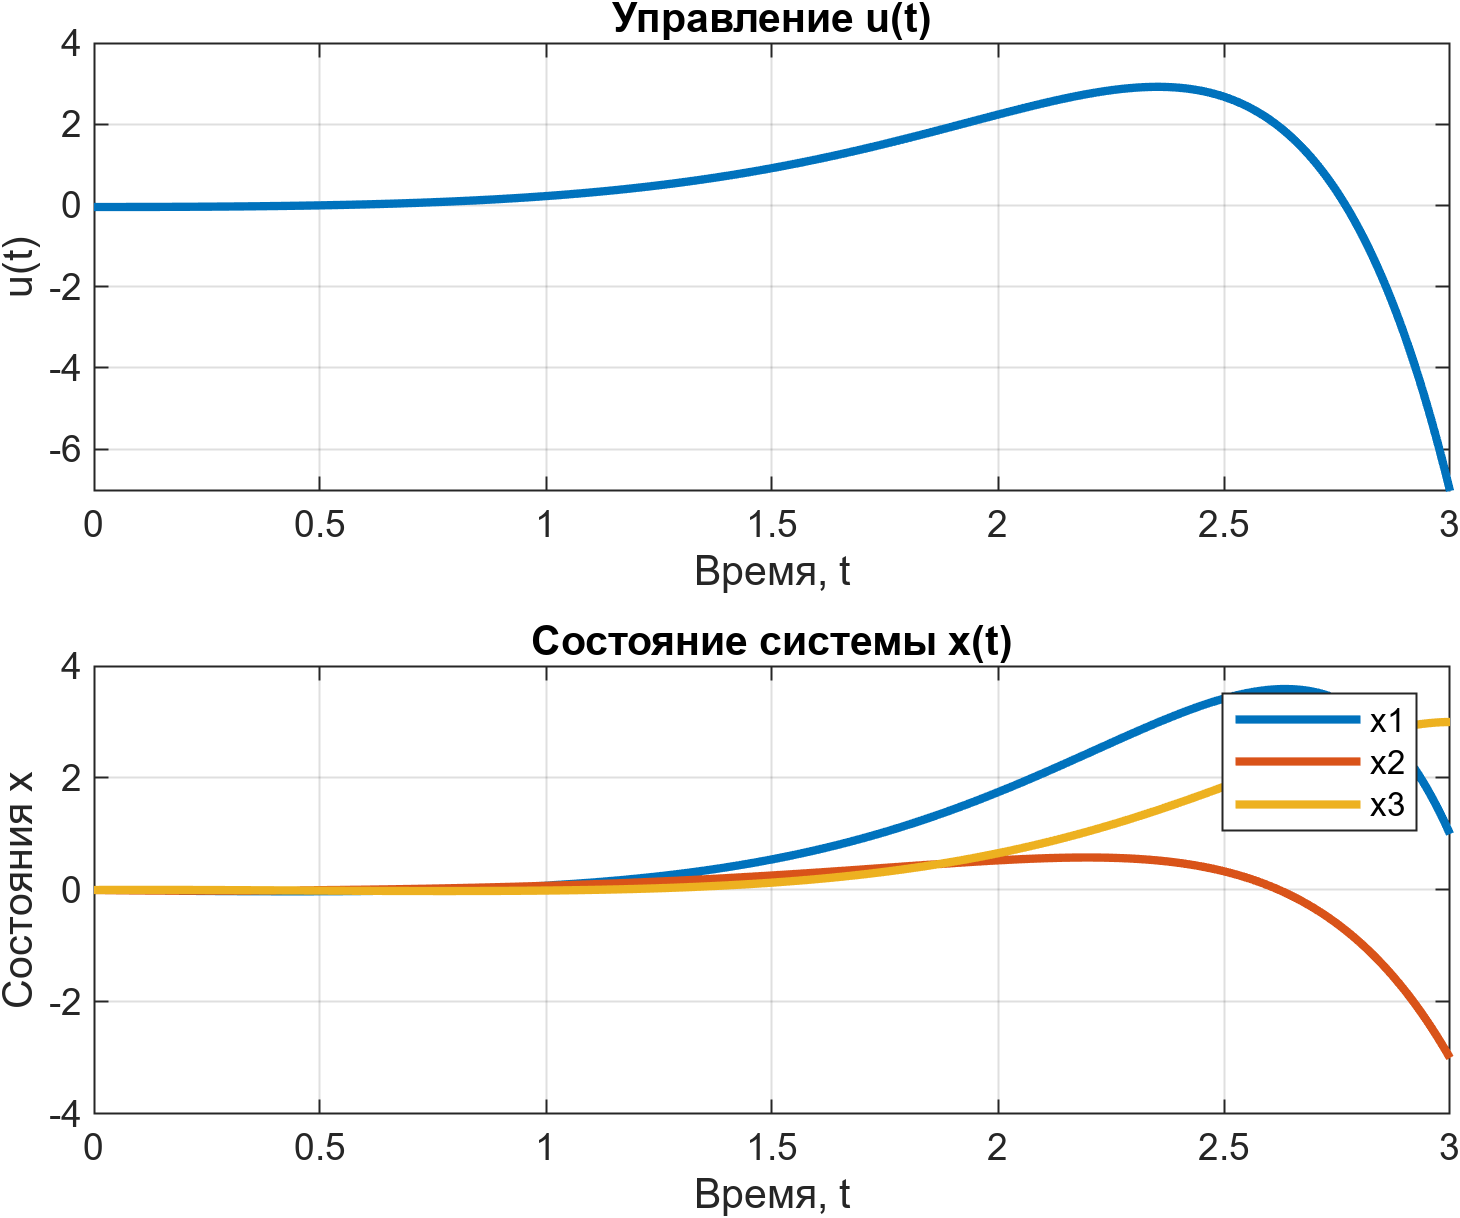
\includegraphics[width=0.7\textwidth]{figs/task_1.png}
    \caption{Система с программным управлением}
    \label{fig:task1}
\end{figure}
Как видно, система переводится в состояние $x_1$ за время $t_1=3$.

\subsection{Вывод}

На основе трех критериев (матрица управляемости, критерий Хаутуса и жорданова форма) 
было установлено, что система полностью управляема. 
Также был найден грамиан управляемости и определено программное управление, 
которое переводит систему из начального состояния в заданное за время $t_1=3$. 
Результаты моделирования показали, что найденное управление позволяет точно перевести систему в требуемое состояние.



\section{Еще одно исследование управляемости}

Рассматриваем систему:
\begin{equation*}
    \dot x=Ax+Bu,\quad
    A=\begin{bmatrix}
        -1 & 1 & 0 \\ -2 & -4 & -1 \\ 2 & 2 & -1
    \end{bmatrix},\quad
    B=\begin{bmatrix}
        2 \\ -1 \\ 1
    \end{bmatrix},\quad
    x_1'=\begin{bmatrix}
        1 \\ -3 \\ 3
    \end{bmatrix},\quad
    x_1''=\begin{bmatrix}
        0\\-2\\3
    \end{bmatrix}.
\end{equation*}

\subsection{Проверка точек}

Если состояние $x_1$ принадлежит управляемому множеству, то
\begin{equation*}
    rank\ U=rank\ [U\ x_1].
\end{equation*}
Проверим данные состояния $x_1'$ и $x_1''$:
\begin{equation*}
    [U\ x_1']=
    \begin{bmatrix}
        2 & -3 & 2 & 1\\
        -1 & -1 & 9 & -3\\
        1 & 1 & -9 & 3
    \end{bmatrix};\quad
    [U\ x_1'']=
    \begin{bmatrix}
        2 & -3 & 2 & 0\\
        -1 & -1 & 9 & -2\\
        1 & 1 & -9 & 3
    \end{bmatrix}.
\end{equation*}
Первая матрица имеет ранг 2, а вторая 3. Если посмотреть чуть ниже на ранг матрицы управляемости,
то делаем вывод, что только $x_1'$ принадлежит управляемому пространству. Это состояние будет
целевым $x_1=x_1'$.

\subsection{Исследование управляемости}

Найдем матрицу управляемости:
\begin{equation*}
    U=[B\quad AB\quad A^2B]=
    \begin{bmatrix}
        2 & -3 & 2 \\ -1 & -1 & 9 \\ 1 & 1 & -9
    \end{bmatrix}.
\end{equation*}
Матрица имеет ранг 2, следовательно \textbf{система неуправляема}.

Спектр матрицы $A$:
$$\sigma(A)=\{ -2 + j;\ -2-j;\ -2\},$$
тогда матрицы Хаутуса ($[A-\lambda_iI\quad B]$) соответственно:
\begin{equation*}
    \begin{bmatrix}
        1-j&1&0&2\\
        -2&-2-j&-1&-1\\
        2&2&1-j&1
    \end{bmatrix},\quad 
    \begin{bmatrix}
        1+j&1&0&2\\-2&-2+j&-1&-1\\2&2&1+j&1
    \end{bmatrix},\quad
    \begin{bmatrix}
        1 & 1 & 0 & 2 \\
        -2 & -2 & -1 & -1 \\
        2 & 2 & 1 & 1
    \end{bmatrix}.
\end{equation*}
Первые две матрицы трехранговые, что делает комплексно сопряженные корни
\textbf{управлемыми}, но а вот третья матрица имеет ранг 2, следовательно собственное
число $-2$ \textbf{неуправляемо}. Значит система не управлема.

Жорданова форма матрицы $A$ и $P^{-1}B$:
\begin{equation*}
    A =\begin{bmatrix}
        
-2&	   0&	   0\\
0&	  -2&	   -1\\
0&	   1&	  -2\\

    \end{bmatrix},\quad
    P^{-1}B=\begin{bmatrix}
        0 \\ 0.7071 \\ -2.1213
    \end{bmatrix}.
\end{equation*}
Как видно, одна из клеток не управляема, а значит и \textbf{исходная система
неуправляема}.

Итого, все три критерия сошлись на том, что система не управляема.

\subsection{Грамиан}

Найдем Грамиан управляемости системы относительно времени $t_1=3$:
\begin{equation*}
    P(3)=\int_{0}^{3}e^{At}BB^Te^{A^Tt}dt=
    \begin{bmatrix}
        1.1250  & -0.8750   & 0.8750\\
        -0.8750  &  0.7500 &  -0.7500\\
         0.8750   &-0.7500&    0.7500
    \end{bmatrix}.
\end{equation*}
Его спектр:
\begin{equation*}
    \sigma(P(3))=\{ 2.5640;\ 
    0.0609;\ 
    0.0000\},
\end{equation*}
одно число нулевое, а значит Грамиан вырожден и программное управление честно найти не представлется
возможным. Будем использовать псевдообратную матрицу:
\begin{equation*}
    P(3)^+=\begin{bmatrix}
        9.6001&    5.6001  & -5.6001\\
        5.6001 &   3.6000 &  -3.6000\\
       -5.6001  & -3.6000&    3.6000
    \end{bmatrix}.
\end{equation*}

\subsection{Управление}

Чтобы перевести систему из $x(0)=0$ в $x(3)=x_1$, возьмем программное управление:
\begin{multline*}
    u(t) = B^T e^{A^T(3 - t)} P(3)^+ x_1 = \\ =
    \begin{bmatrix}
        2 & -1 & 1
    \end{bmatrix}\cdot
    \exp\left( 
    \begin{bmatrix}
        -1&  1 & 0\\
        -2 &-4& -1\\
        2  &2& -1
    \end{bmatrix}\cdot(3 - t) \right)\cdot
    \begin{bmatrix}
        9.6001&    5.6001  & -5.6001\\
        5.6001 &   3.6000 &  -3.6000\\
       -5.6001  & -3.6000&    3.6000
    \end{bmatrix}\cdot
    \begin{bmatrix}
        1 \\ -3 \\ 3
    \end{bmatrix}=\\
    =-e^{2t-6}\left(16.0012\cos\left(t-3\right)+71.9989\sin\left(t-3\right)\right).
\end{multline*}
Смоделируем систему и данное управление, результаты приведены на рисунке \ref{fig:task2}.
\begin{figure}[H]
    \centering
    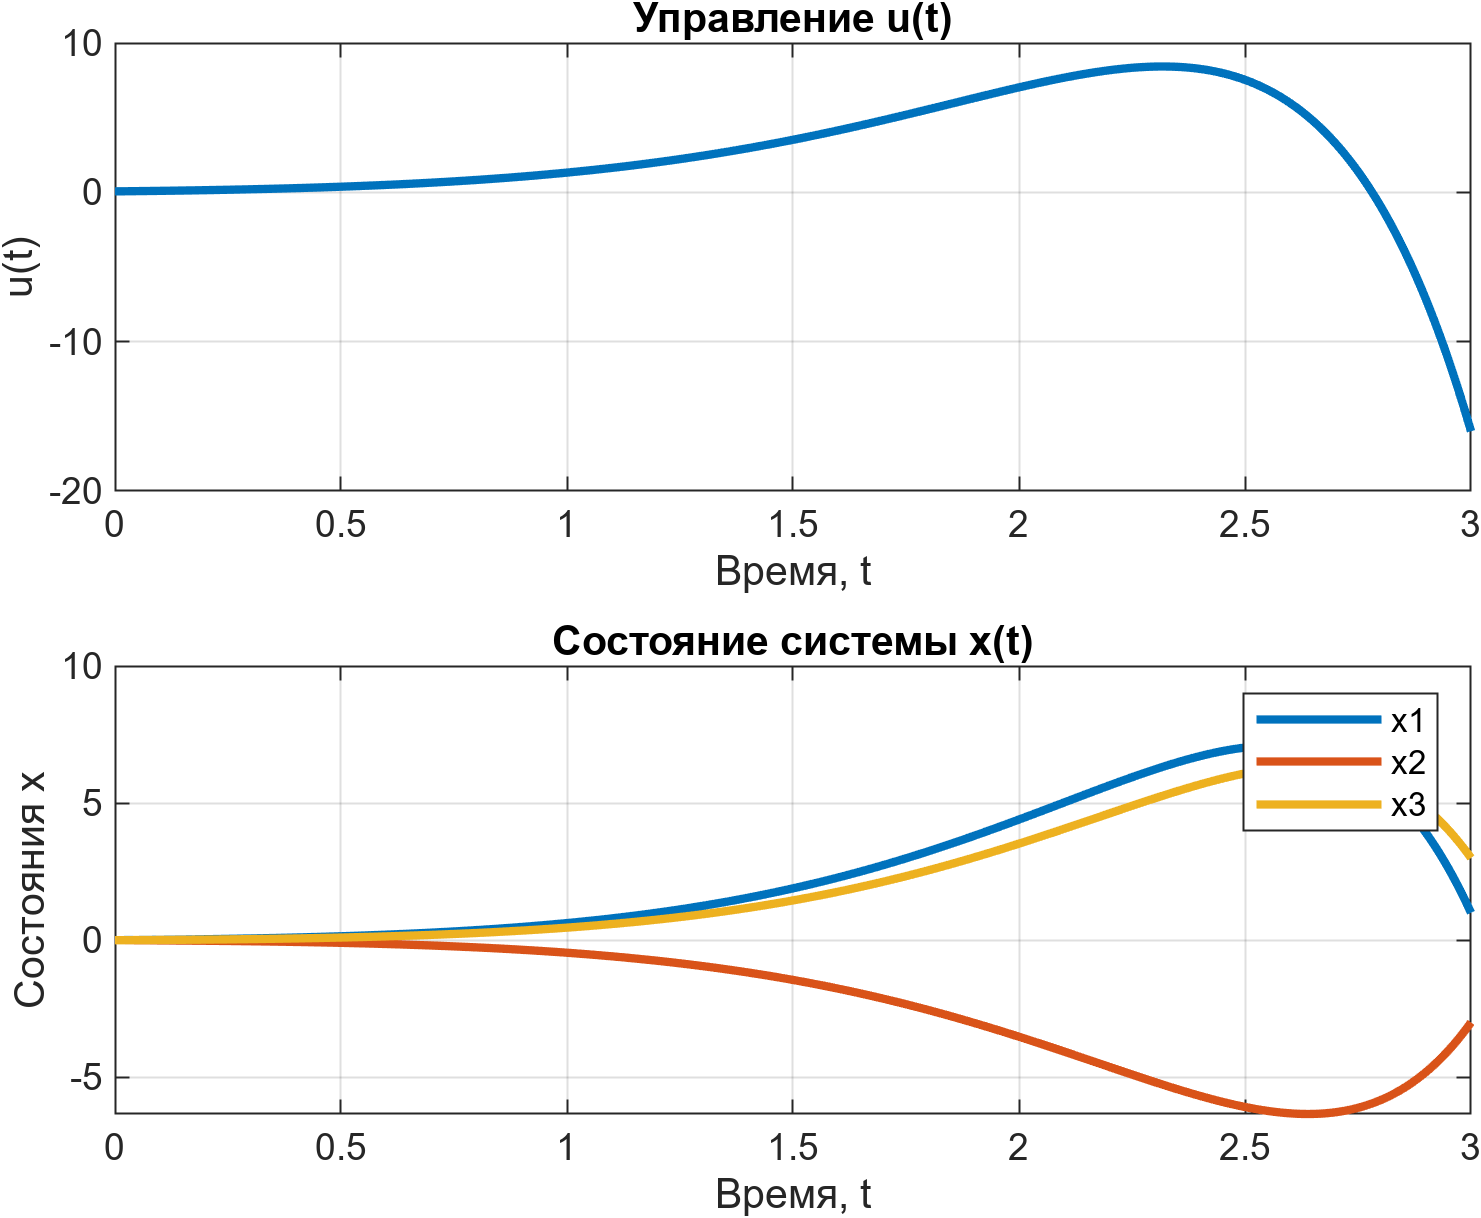
\includegraphics[width=0.7\textwidth]{figs/task_2.png}
    \caption{Система с "псевдо программным" управлением}
    \label{fig:task2}
\end{figure}
Как видно, система переводится в состояние $x_1$ за время $t_1=3$.

\subsection{Вывод}

В итоге, по всем критериям система неуправляема. Однако для состояния из управляемого пространства было найдено управление.



\section{Исследование наблюдаемости}

Рассматриваем систему:
\begin{equation*}
    \begin{cases}
        \dot x = Ax\\
        y = Cx
    \end{cases},\quad
    A = \begin{bmatrix}
        -21 & -38 & 6 \\
        8 & 13 & -4 \\
        -6 & -14 & -1
    \end{bmatrix},\quad
    C = \begin{bmatrix}
        9 & 18 & -2
    \end{bmatrix},
\end{equation*}
и функцию
\begin{equation*}
    f(t)=3e^{-5t} cos(2t) - e^{-5t} sin(2t).
\end{equation*}

\subsection{Исследование наблюдаемости}

Матрица наблюдаемости системы
\begin{equation*}
    V=\begin{bmatrix}
        C \\ CA \\ CA^2
    \end{bmatrix}
    =\begin{bmatrix}
        9 & 18 & -2 \\
        -33 & -80 & -16 \\
        149 & 438 & 138
    \end{bmatrix}.
\end{equation*}
Она имеет ранг 3, из чего следует, что \textbf{система полностью наблюдаема}. Собственные
числа системы - $\sigma(A)=\{1;\ -5+j2;\ -5-j2\}$. Соответственно,
матрицы Хаутуса:
\begin{equation*}
    \begin{bmatrix}
        -22&	-38&	6\\
        8&	12&	-4\\
        -6&	-14&	-2\\
        9&	18&	-2
    \end{bmatrix},\quad
    \begin{bmatrix}
        -16 - 2i&	-38&	6\\
        8&	18 - 2i&	-4\\
        -6&	-14&	4 - 2i\\
        9&	18&	-2
    \end{bmatrix},\quad
    \begin{bmatrix}
        -16 + 2i&	-38&	6\\
8&	18 + 2i&	-4\\
-6&	-14&	4 + 2i\\
9&	18&	-2
    \end{bmatrix}.
\end{equation*}
Матрицы Хаутуса имеют ранг 3, что означает, что все собственные
числа наблюдаемы, а значит и \textbf{вся система наблюдаема}.
Вещественная жордановая форма матрицы $A$ и новая $C'=C\cdot P$:
\begin{equation*}
    A = \begin{bmatrix}
        2.0000&    4.2426   &-2.8284\\
        -1.0000&   -1.4142 &   1.4142\\
         1.0000 &   1.4142&         0
    \end{bmatrix}\cdot
    \begin{bmatrix}
        1&     0  &   0\\
        0 &   -5 &   -2\\
        0  &   2&    -5
    \end{bmatrix}\cdot
    \begin{bmatrix}
        -1.0000&   -2.0000 &   1.0000\\
        0.7071  &  1.4142 &        0\\
             0   & 0.7071&    0.7071\\
    \end{bmatrix},
\end{equation*}
\begin{equation*}
    C\cdot P=\begin{bmatrix}
        -2.0000 & 9.8995 & 0
    \end{bmatrix}.
\end{equation*}
Как видно, каждое собственное число наблюдаемо, и, как следствие,
\textbf{исходная система полностью наблюдаема}.

В итоге, все три критерия сошлись на том, что система полностью
наблюдаема.

\subsection{Грамиан наблюдаемости}

Грамиан наблюдаемости системы относительно времени $t_1 = 3$:
\begin{equation*}
    Q(3)=\int\limits_{0}^{3}e^{A^Tt}C^TCe^{At}dt=10^3\cdot\begin{bmatrix}
        0.8150&    1.6278  & -0.8099\\
        1.6278 &   3.2514 &  -1.6181\\
       -0.8099  & -1.6181&    0.8080
    \end{bmatrix}.
\end{equation*}
Его собственные числа:
\begin{equation*}
    \sigma(Q(3))=\{4872.0;\ 0.1;\ 2.4\}.
\end{equation*}
Все собственные числа ненулевые, а значит Грамиан невырожден и можно однозначно
вычислить начальные условия.

\begin{figure}[H]
    \centering
    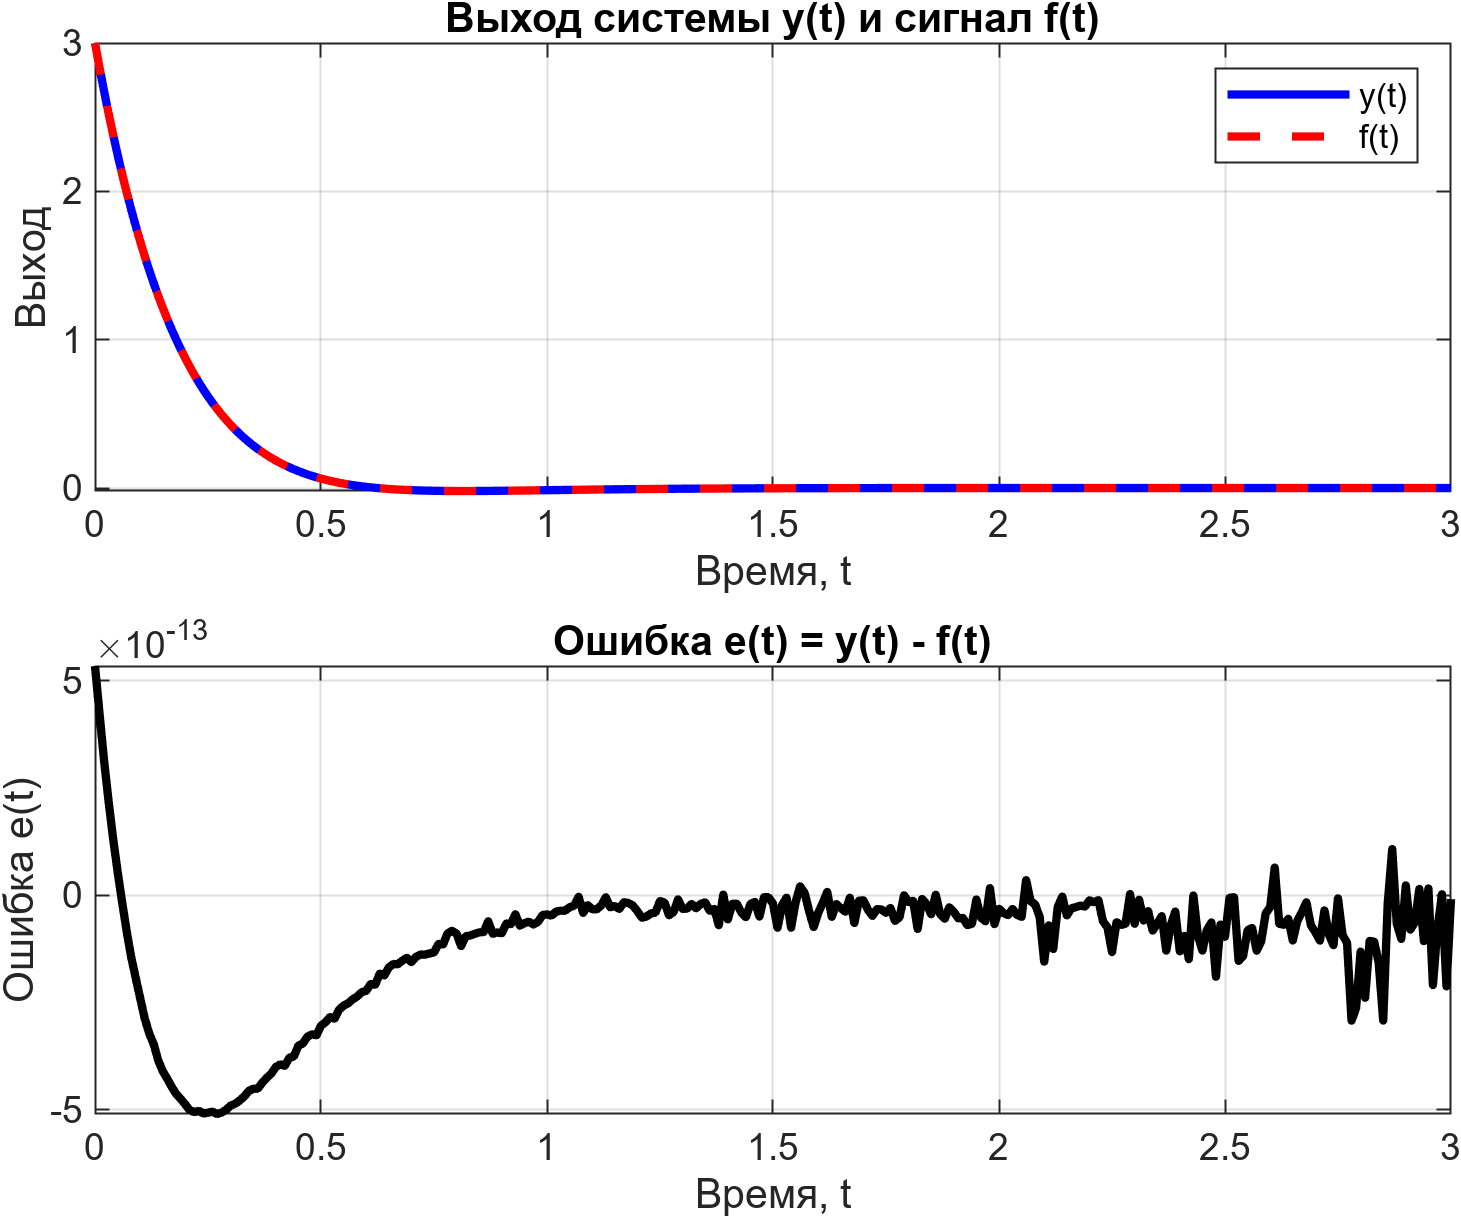
\includegraphics[width=0.7\textwidth]{figs/task_3.png}
    \caption{Система с восстановленными начальными условиями}
    \label{fig:task3}
\end{figure}

\subsection{Начальные условия}

Считая, что выход системы $y(t)$ подчиняется закону $y(t) = f (t)$ на временном
интервале $t \in [0, t_1]$ определим начальные условия системы:
\begin{equation*}
    x(0)=Q^{-1}(3)\int\limits_{0}^{3}e^{A^Tt}C^Ty(t)dt
    =\begin{bmatrix}
        1.0000 \\ -0.2857 \\ 0.4286
    \end{bmatrix}.
\end{equation*}
Со знанием начальных условий можно восстановить всю траекторию
$x(t)=e^{At}x(0)$. Смоделируем систему, на рисунке \ref{fig:task3}
приведены выход системы, сигнал $f(t)$ и ошибка, как видно, все сходится.

\subsection{Вывод}

На основе трех критериев было установлено, 
что система полностью наблюдаема. Также был найден грамиан наблюдаемости и определены 
начальные условия системы. Результаты моделирования показали, что восстановленные 
начальные условия позволяют точно воспроизвести траекторию системы.



\section{Еще одно исследование наблюдаемости}

Рассматриваем систему:
\begin{equation*}
    \begin{cases}
        \dot x = Ax\\
        y = Cx
    \end{cases},\quad
    A = \begin{bmatrix}
        -21 & -38 & 6 \\
        8 & 13 & -4 \\
        -6 & -14 & -1
    \end{bmatrix},\quad
    C = \begin{bmatrix}
        7 & 14 & 0
    \end{bmatrix},
\end{equation*}
и функцию
\begin{equation*}
    f(t)=3e^{-5t} cos(2t) - e^{-5t} sin(2t).
\end{equation*}

\subsection{Исследование наблюдаемости}

Матрица наблюдаемости системы
\begin{equation*}
    V=\begin{bmatrix}
        C \\ CA \\ CA^2
    \end{bmatrix}
    =\begin{bmatrix}
        7&	14&	0\\
        -35&	-84&	-14\\
        147&	434&	140
    \end{bmatrix}.
\end{equation*}
Она имеет ранг 2, из чего следует, что \textbf{система ненаблюдаема}. 
Собственные
числа системы - $\sigma(A)=\{1;\ -5+j2;\ -5-j2\}$. Соответственно,
матрицы Хаутуса:
\begin{equation*}
    \begin{bmatrix}
        -22&	-38&	6\\
        8&	12&	-4\\
        -6&	-14&	-2\\
        7 & 14 & 0
    \end{bmatrix},\quad
    \begin{bmatrix}
        -16 - 2i&	-38&	6\\
        8&	18 - 2i&	-4\\
        -6&	-14&	4 - 2i\\
        7 & 14 & 0
    \end{bmatrix},\quad
    \begin{bmatrix}
        -16 + 2i&	-38&	6\\
8&	18 + 2i&	-4\\
-6&	-14&	4 + 2i\\
7 & 14 & 0
    \end{bmatrix}.
\end{equation*}
Первая мартица Хаутуса двуранговая, а остальные две трехранговые, что делает
комплексно сопряженные корни \textbf{наблюдаемыми}, но вот собственное число
$1$ \textbf{ненаблюдаемым}. Значит \textbf{система ненаблюдаема}.
Вещественная жордановая форма матрицы $A$ и новая $C'=C\cdot P$:
\begin{equation*}
    A = \begin{bmatrix}
        2.0000&    4.2426   &-2.8284\\
        -1.0000&   -1.4142 &   1.4142\\
         1.0000 &   1.4142&         0
    \end{bmatrix}\cdot
    \begin{bmatrix}
        1&     0  &   0\\
        0 &   -5 &   -2\\
        0  &   2&    -5
    \end{bmatrix}\cdot
    \begin{bmatrix}
        -1.0000&   -2.0000 &   1.0000\\
        0.7071  &  1.4142 &        0\\
             0   & 0.7071&    0.7071\\
    \end{bmatrix},
\end{equation*}
\begin{equation*}
    C\cdot P=\begin{bmatrix}
        0 & 9.8995 & 0
    \end{bmatrix}.
\end{equation*}
Как видно, вещественное собственное число ненаблюдаемо, и, как следствие,
\textbf{исходная система ненаблюдаема}.

В итоге, все три критерия сошлись на том, что система ненаблюдаема.

\subsection{Грамиан наблюдаемости}

Грамиан наблюдаемости системы относительно времени $t_1 = 3$:
\begin{equation*}
    Q(3)=\int\limits_{0}^{3}e^{A^Tt}C^TCe^{At}dt=10^3\cdot\begin{bmatrix}
        4.5621&    8.2793  & -0.8448\\
        8.2793 &  15.2069 &  -1.3517\\
       -0.8448  & -1.3517&    0.3379
    \end{bmatrix}.
\end{equation*}
Его собственные числа:
\begin{equation*}
    \sigma(Q(3))=\{19.8567;\ 0.0000;\ 0.2502\}.
\end{equation*}
Присутствует нулевое собственное число, а значит Грамиан вырожден и
нельзя однозначно вычислить начальные условия. Но попробуем их
вычислить с помощью псевдообратной матрицы.

\begin{figure}[H]
    \centering
    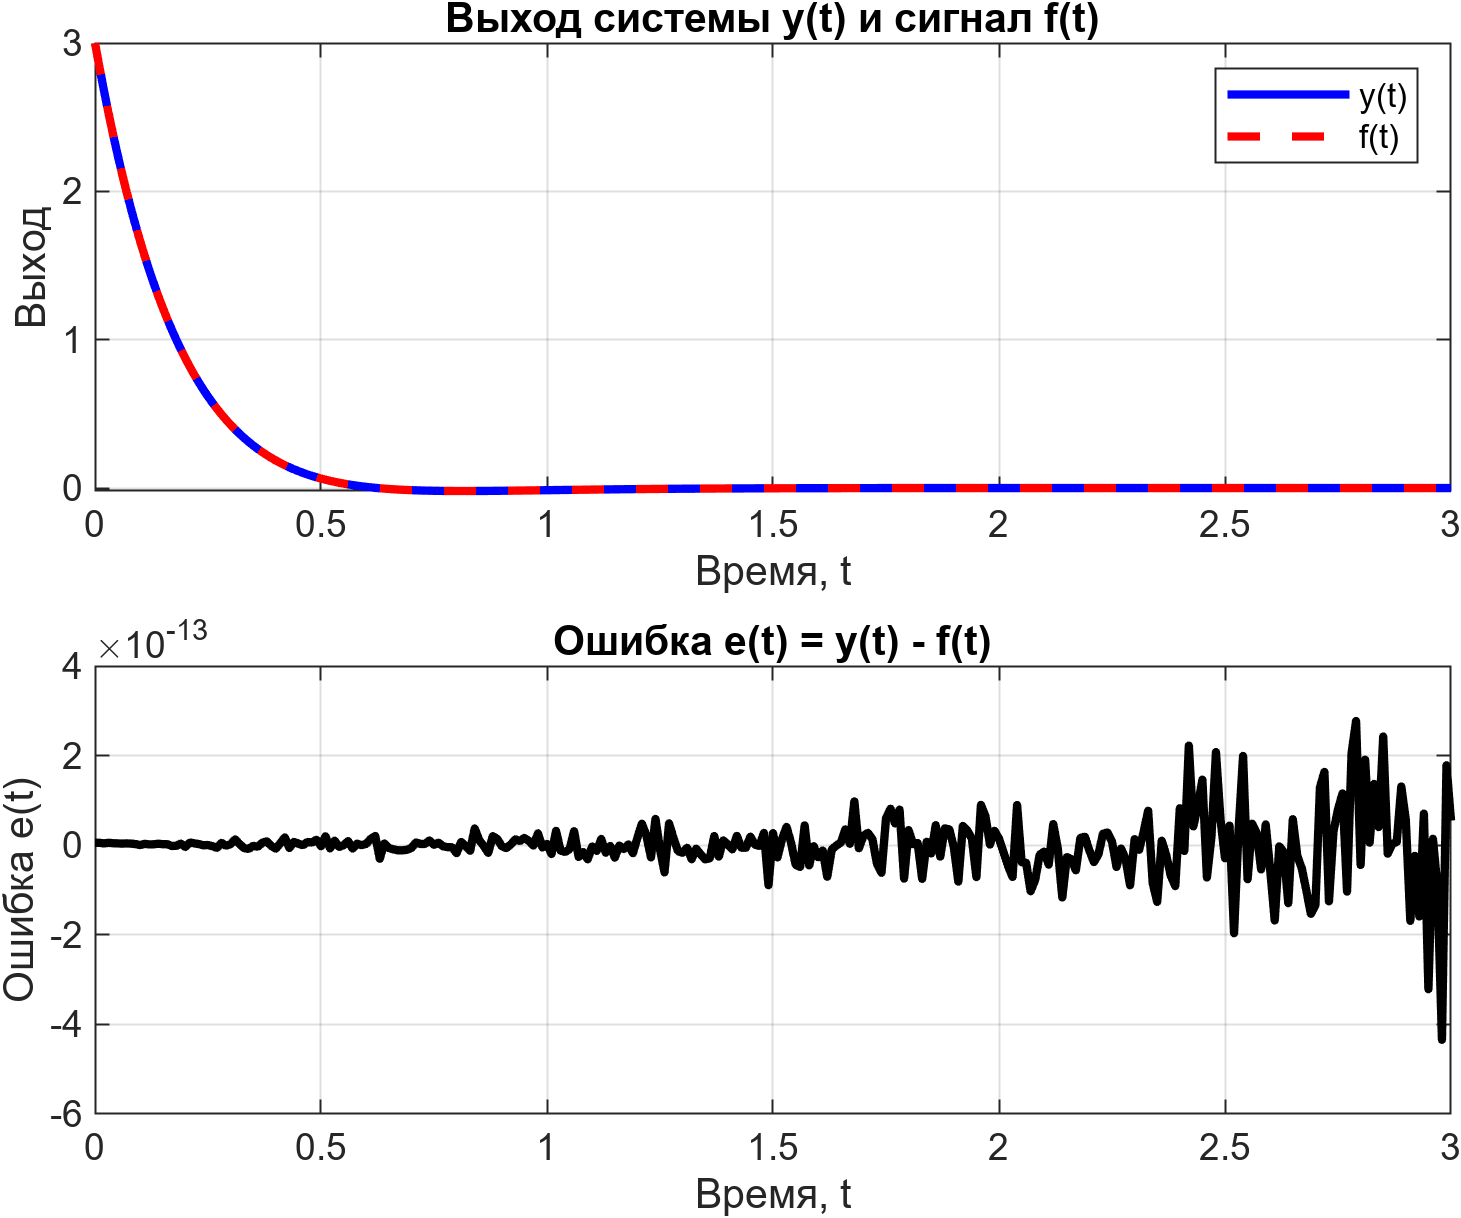
\includegraphics[width=0.7\textwidth]{figs/task_4.png}
    \caption{Система с восстановленными начальными условиями}
    \label{fig:task4}
\end{figure}

\subsection{Начальные условия}

Считая, что выход системы $y(t)$ подчиняется закону $y(t) = f (t)$ на временном
интервале $t \in [0, t_1]$ определим начальные условия системы:
\begin{equation*}
    x(0)=Q^{+}(3)\int\limits_{0}^{3}e^{A^Tt}C^Ty(t)dt
    =\begin{bmatrix}
        0.0952 \\ 0.1667 \\ -0.0238
    \end{bmatrix}.
\end{equation*}
Смоделируем систему, на рисунке \ref{fig:task4}
приведены выход системы, сигнал $f(t)$ и ошибка, как видно, все сходится.

\subsection{Другие начальные условия}

Выход вида $y(t) = f (t)$ может быть порожден начальными условиями, 
отличными от найденных. Найдем их с помощью ядра матрицы наблюдаемости,
базис которого можно найти с помощью MATLAB:
\begin{equation*}
    Nullspace\ V=Span\Big\{\begin{bmatrix}
        0.8165 \\ -0.4082 \\ 0.4082
    \end{bmatrix}\Big\},
\end{equation*}
и, добавив любой вектор из ядра к начальным условиям, $y(t)$
не должна измениться. Проверим это, смоделировав систему, для
этого выберем три новых начальных условия:
\begin{equation*}
    x_1=\begin{bmatrix}
        0.9117\\
   -0.2416\\
    0.3844
    \end{bmatrix},\quad
    x_2\begin{bmatrix}
        1.7282\\
        -0.6498\\
         0.7927
    \end{bmatrix},\quad
    x_3\begin{bmatrix}
        6.6272\\
        -3.0993\\
         3.2422
    \end{bmatrix}.
\end{equation*}
Как видно на рисунке \ref{fig:task41}, все три новых начальных условия
порождают одинаковый выход, при том что они имеют разные начальные условия.

\begin{figure}[H]
    \centering
    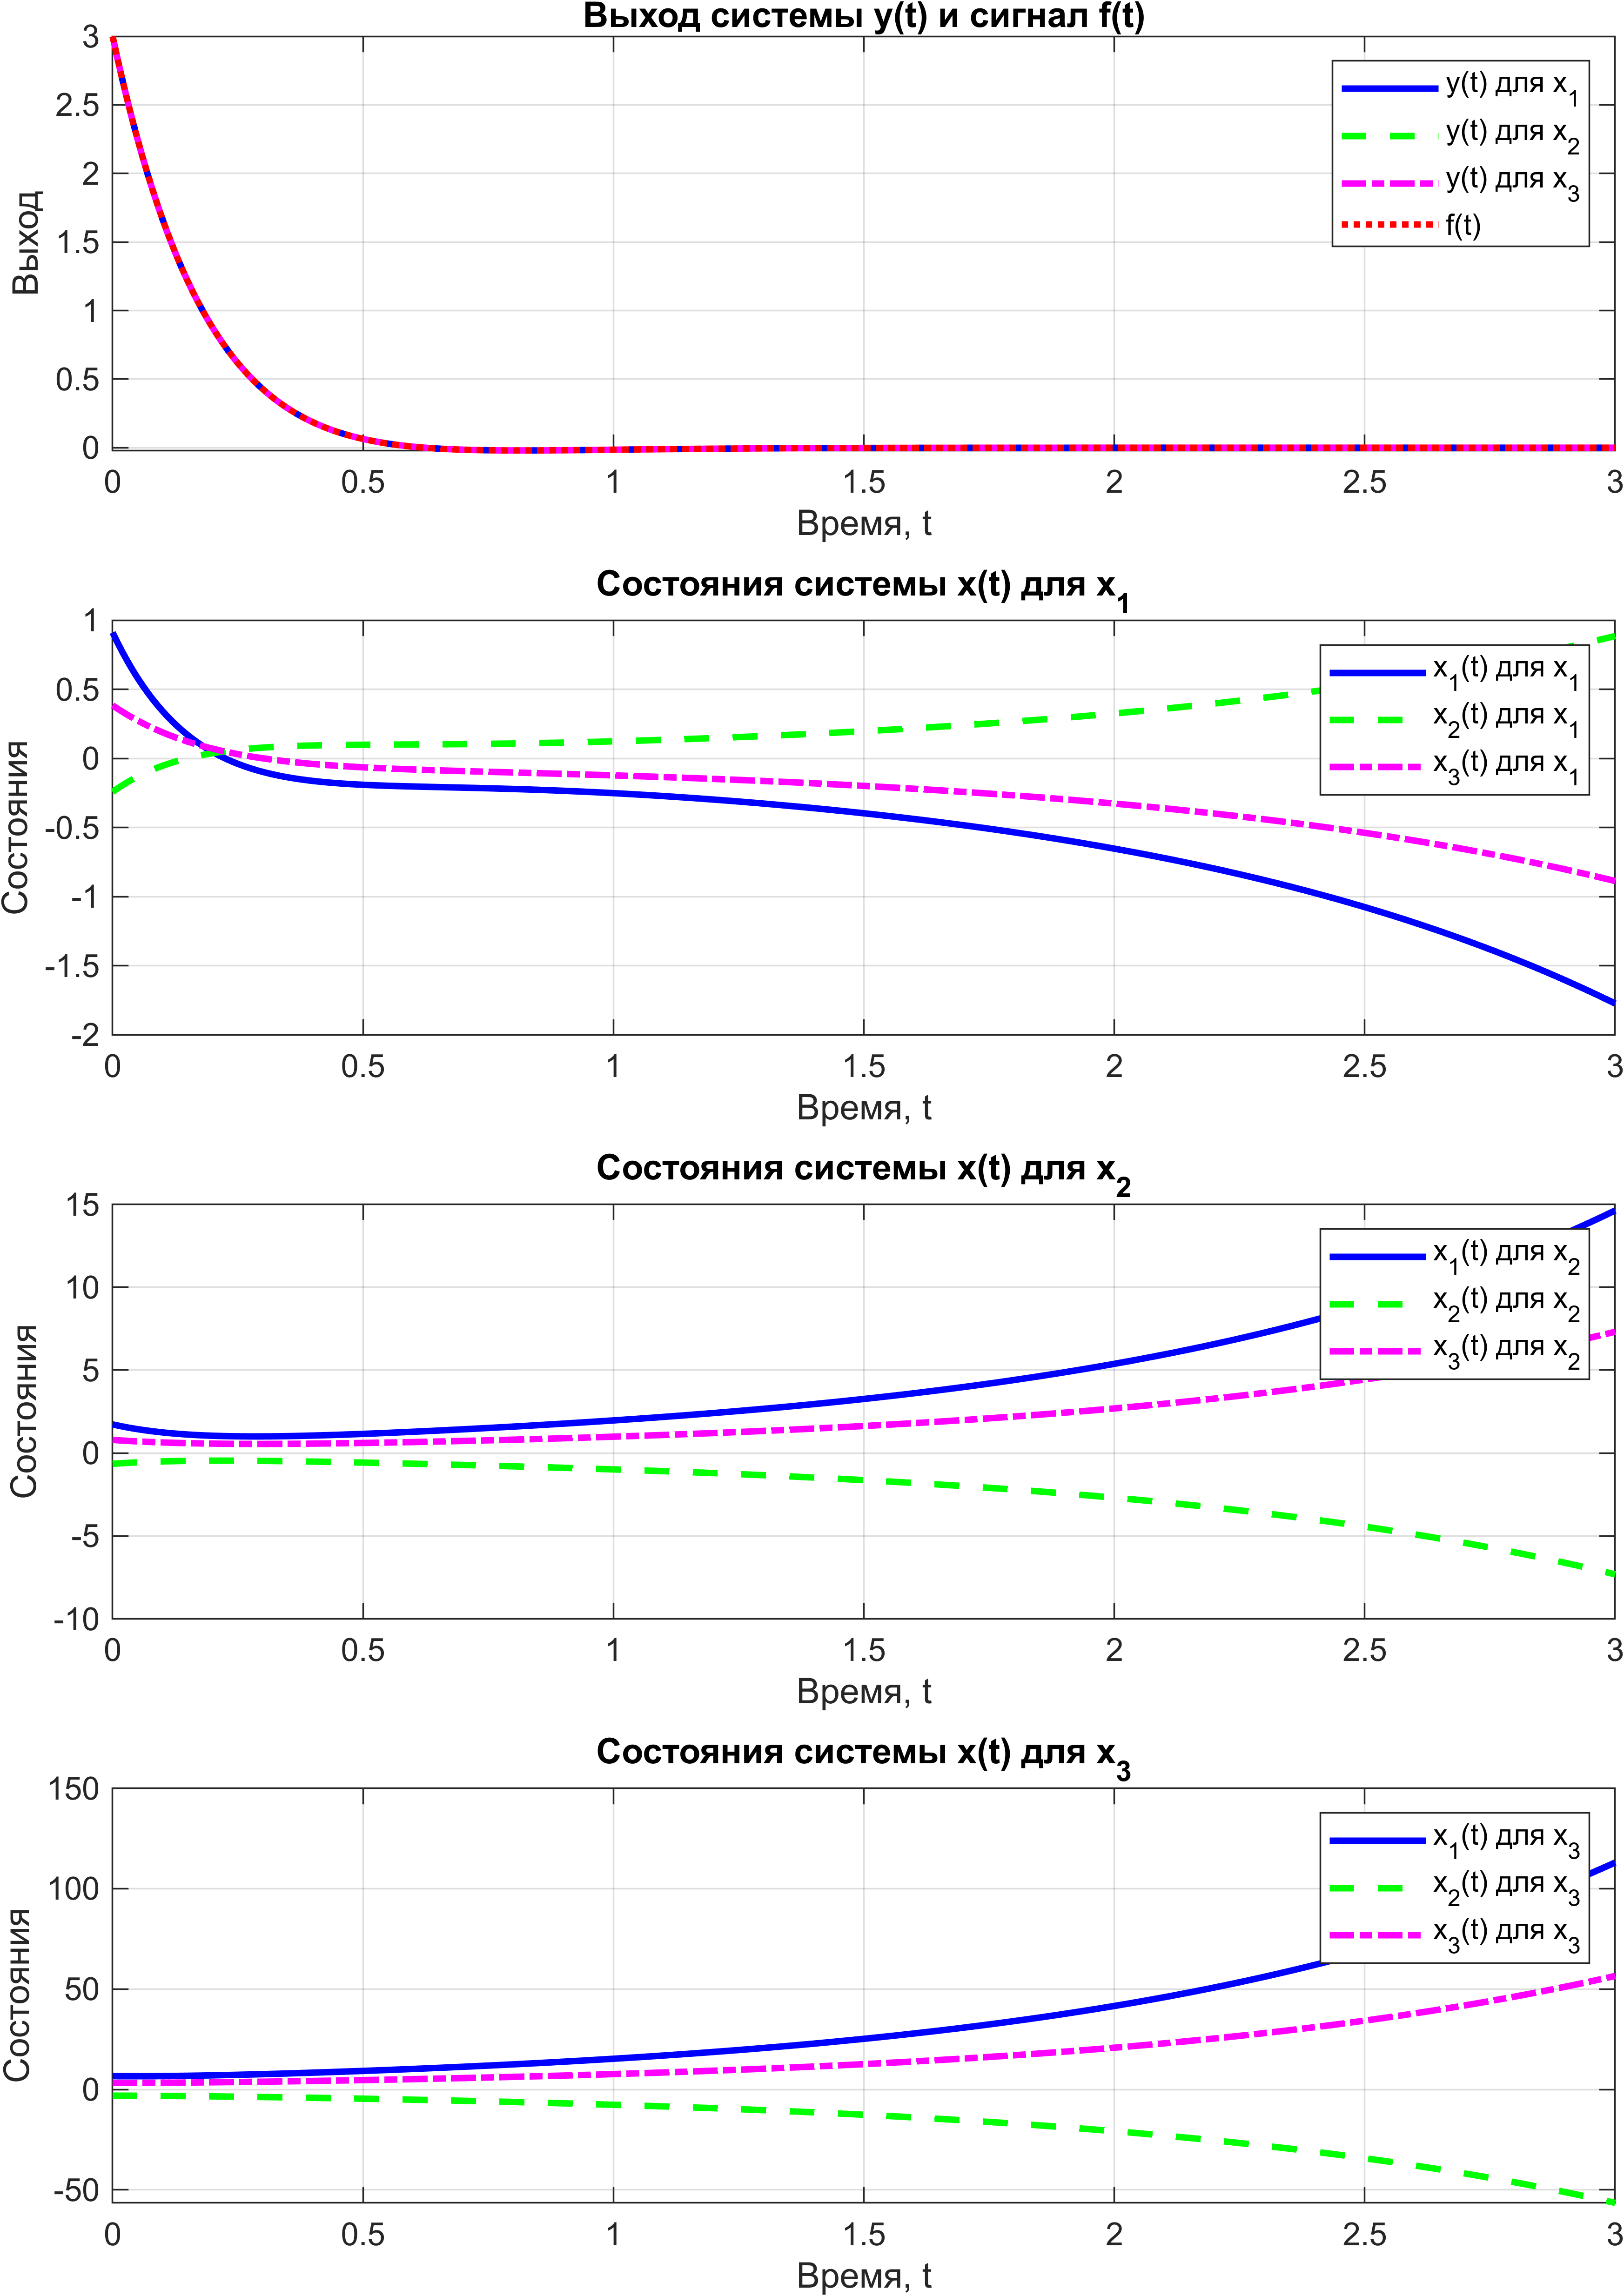
\includegraphics[width=1\textwidth]{figs/task_41.png}
    \caption{Система с другими начальными условиями}
    \label{fig:task41}
\end{figure}

\subsection{Вывод}

На основе трех критериев было установлено, что система ненаблюдаема. 
Также был найден грамиан наблюдаемости и определены начальные условия 
системы с использованием псевдообратной матрицы. Результаты моделирования 
показали, что восстановленные начальные условия позволяют воспроизвести 
траекторию системы. Однако, поскольку система ненаблюдаема, существуют и 
другие начальные условия, которые порождают тот же выход системы.



\section{Исследование управляемости по выходу}

Рассмотрим систему:
\begin{equation*}
    \begin{cases}
        \dot x = Ax + Bu\\
        y = Cx + Du
    \end{cases},\quad
    A=\begin{bmatrix}
        -1 & 1 & 0 \\ -2 & -4 & -1 \\ 2 & 2 & -1
    \end{bmatrix},\quad
    B=\begin{bmatrix}
        2 \\ 3 \\ 1
    \end{bmatrix},\quad
    C=\begin{bmatrix}
        0 & -1 & -2 \\
        0 & 1 & 2
    \end{bmatrix}.
\end{equation*}

Жорданова форма матрицы $A$:
\begin{equation*}
    A=\begin{bmatrix}
        -1.0000&    0.7071 &  -0.7071\\
        1.0000  & -1.4142 &        0\\
             0   & 1.4142&         0
    \end{bmatrix}\cdot
    \begin{bmatrix}
        -2&     0 &    0\\
        0  &  -2 &   -1\\
        0   &  1&    -2
    \end{bmatrix}\cdot
    \begin{bmatrix}
        0&    1.0000  &  1.0000\\
        0 &        0 &   0.7071\\
  -1.4142  & -1.4142&   -0.7071
    \end{bmatrix},
\end{equation*}
новые матрицы $B$ и $C$:
\begin{equation*}
    P^{-1}\cdot B=\begin{bmatrix}
        4.0000\\
        0.7071\\
       -7.7782
    \end{bmatrix},\quad
    C\cdot P=\begin{bmatrix}
        -1.0000&   -1.4142&         0\\
        1.0000  &  1.4142&         0
    \end{bmatrix}.
\end{equation*}
Как видно, исходная система управляема и наблюдаема.

Найдем матрицу управляемости:
\begin{equation*}
    U=[B\quad AB\quad A^2B]=\begin{bmatrix}
        2&	1&	-18\\
        3&	-17&	57\\
        1&	9&	-41
    \end{bmatrix},
\end{equation*}
найдем матрицу управляемости по выходу при $D=0_{2X2}$:
\begin{equation*}
    U_{out}=[C\cdot U\quad D]=\begin{bmatrix}
        -5&    -1&    25&     0&     0\\
        5 &    1&   -25  &   0&     0
    \end{bmatrix}.
\end{equation*}
Ранг данной матрицы единица, что не равно размерности $y$, а значит
\textbf{система неуправляема по выходу}. Это следует из того, что
матрица $C$ имеет неполный ранг, а  ранг произведения не превосходит 
рангов каждого из сомножителей, следовательно, произведение $CU$
тоже имеет неполный ранг, а значит мы не сможем добиться любого выхода
для удовлетворения определения управляемости по выходу. Для исправления
данной ситуации можно изменить матрицу $D$, которую мы принимали нулевой,
нам нужно обеспечить линейную независимость строк матрицы $U_{out}$,
для этого подойдет единичная матрица $D=I_{2X2}$. Теперь
\begin{equation*}
    U_{out}=[C\cdot U\quad D]=\begin{bmatrix}
        -5&    -1&    25&     1&     0\\
        5 &    1&   -25  &   0&     1
    \end{bmatrix},
\end{equation*}
матрица имеет ранг 2, а значит \textbf{система управляема по выходу}.

\subsection{Вывод}

Было установлено, что данная система управляема и наблюдаема, однако
неуправляема по выходу при нулевой матрице $D$. Но, при изменении 
матрицы $D$ на единичную, система становится управляема по выходу. 
Это показывает важность выбора правильной матрицы $D$ для обеспечения 
управляемости по выходу.

\section{Заключение}

В данной лабораторной работе были исследованы вопросы управляемости 
и наблюдаемости линейных систем. Были рассмотрены различные критерии, 
такие как матрица управляемости, критерий Хаутуса, жорданова форма, 
а также грамианы управляемости и наблюдаемости. На основе этих критериев 
были сделаны выводы об управляемости и наблюдаемости систем. 
Также были найдены программные управления и начальные условия для систем, 
что позволило перевести системы в заданные состояния и восстановить 
траектории. В конце, было рассмотрено управление по выходу и показано, 
что правильный выбор матрицы $D$ может существенно повлиять 
на управляемость системы по выходу.